\section{Misure di un impedenza tramite ponte di Wien}

\begin{wrapfigure}[15]{r}[0pt]{80mm}
	\centering
    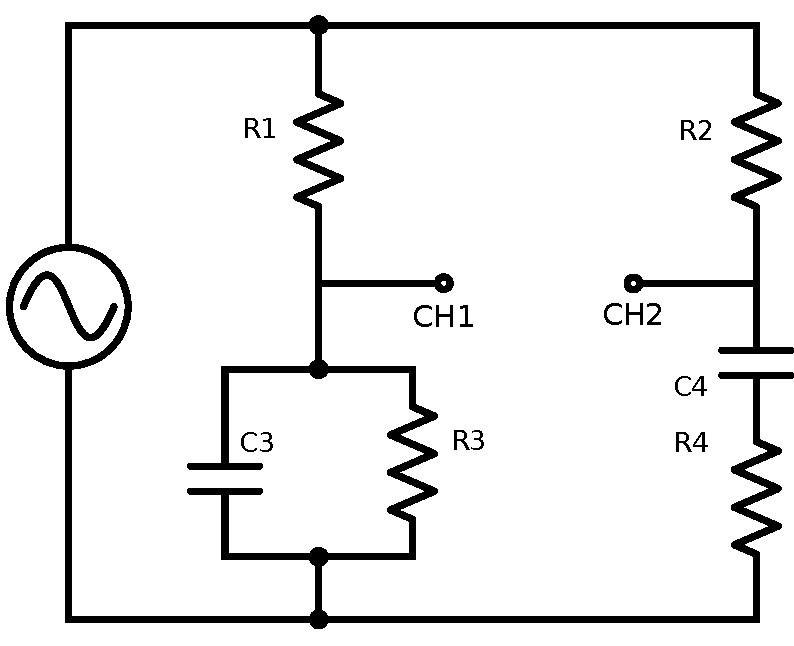
\includegraphics[width=0.30\textwidth]{schema1.pdf}
    \caption{Schema del circuito utilizzato per la misura di impedenza.}
    \label{fig:circuito1}
\end{wrapfigure}

\subsection{Acquisizione dati}
Una volta montato il circuito e collegato al generatore di forme d'onda sono stati collegati i due canali dell'oscilloscopio alle uscite del circuito (CH1 e CH2, come in Figura \ref{fig:circuito1}). 
\`E stata fissata una tensione di $5\,Vpp$ e, dopo aver stabilizzato con il comando $trigger$ le forme d'onda sullo schermo e averle allineate, sono state impostate le funzioni integrate dell'oscilloscopio che permettevano di ricavare valori più stabili e meno affetti da rumore tramite la media di più misure.

Per calcolare il valore di capacità del condensatore incognito $C_3$ è stato necessario bilanciare il ponte. Ciò significa variare gli elementi circuitali, nel nostro caso $R_1$ (la decade di resistenze) e la frequenza $\omega$ a cui veniva generata la \emph{ddp} dal generatore finché i segnali che l'oscilloscopio leggeva da CH1 e CH2 fossero stati i medesimi.

Lavorando sulla frequenza e sulla resistenza abbiamo cercato quindi di bilanciare il circuito in modo tale che, in ogni momento, lo sfasamento tra CH1 e CH2 fosse nullo e l'ampiezza di segnale identica. Così facendo, infatti, a qualsiasi instante di tempo $t, \,\,\,\, V(CH1)=V(CH2)$, ovvero il ponte risulta essere bilanciato. 

\subsection{Analisi dati}

La frequenza e la resistenza necessarie per bilanciare il ponte si sono rivelate essere:

\begin{equation*}
\omega \, = 2 \, \pi \, \nu \, = \, 2 \, \pi \, (2762.2 \pm 0.1) \, \si{\hertz}
\qquad R_1 \, = \, (14389 \pm 1) \, \si{\ohm}
\end{equation*}


\noindent Quindi, utilizzando le equazioni di bilanciamento \ref{eq:1bilanciamento} e \ref{eq:2bilanciamento}:\\

\noindent
\begin{minipage}{.5\linewidth}

\begin{equation}
\frac{R_4}{R_3} + \frac{C_3}{C_4} = \frac{R_2}{R_1}
\label{eq:1bilanciamento}
\end{equation}

\end{minipage}%
\begin{minipage}{.5\linewidth}

\begin{equation}
\omega^2 \, R_3 \, C_3 \, R_4 \, C_4 \, = \, 1
\label{eq:2bilanciamento}
\end{equation}

\end{minipage}

si ottiene:

\begin{equation}
C_3 \, = \, \frac{C_4 \, R_2}{R_1 \, (1 \, + \, \omega^2 \, R_4^2 \, C_4^2)}
\label{eq:C3}
\end{equation}

Ricordiamo che i valori di resistenze e di capacità noti del circuito erano:\\
I valori da noi ottenuti per la capacità incognita sono stati\footnote{Valori di resistenze e capacità sono stati misurati utilizzando il multimetro digitale, che permette misure più precise. Per stimare gli errori sui dati calcolati analiticamente sono state sfruttate le formule di propagazione degli errori}\\

%\begin{SCtable}[20]
%\centering
%\caption{In tabella sono riportati i valori della capacità incognita $C_3$ calcolati mediante le tre formule sopra riportate e il multimetro a nostra disposizione.}
%\begin{tabular}{m{75pt}|m{48pt}|m{48pt}|m{48pt}|m{48pt}}
%\vspace{12pt} & multimetro\\&hai & Eq. \ref{eq:1bilanciamento} & Eq. \ref{eq:2bilanciamento} & Eq. \ref{eq:C3} \\
%\hline
%\vspace{0pt} & & & &\\
%\vspace{8pt} \centering Capacità $C_3$ [$\si{\nano\farad}$] & \vspace{8pt} \centering $(3.4 \pm 0.1)$ & \vspace{8pt} \centering $(3.7 \pm 0.2)$ & \vspace{8pt} \centering $(3.5 \pm 0.2)$ & \vspace{8pt} \centering ($3.5 \pm 0.1$)
%\label{tab:C}
%\end{tabular}
%\end{SCtable}

\begin{SCtable}[20]
\centering
\caption{In tabella sono riportati i valori della capacità incognita $C_3$ calcolati mediante le tre formule sopra riportate e il multimetro a nostra disposizione.}
{\renewcommand{\arraystretch}{1.6}%
\begin{tabular}{c|c|c|c|c}
 & multimetro & Eq. \ref{eq:1bilanciamento} & Eq. \ref{eq:2bilanciamento} & Eq. \ref{eq:C3} \\      \hline
Capacità $C_3$ [$\si{\nano\farad}$] & $(3.4 \pm 0.1)$ & $(3.7 \pm 0.2)$ & $(3.5 \pm 0.2)$ & ($3.5 \pm 0.1$) \\
\end{tabular}}
\end{SCtable}

Come vediamo, i valori ottenuti con tutti e tre i calcoli si rivelano compatibili con il valore misurato dal multimetro. Ci siamo informati sul valore di capacità fornito dal costruttore ed esso risulta essere $(3.3 	\pm 0.3 )\si{\pico\farad}$. Notiamo come la terza procedura (quella che tiene conto sia di $R1$ che di $\omega$) sia la più precisa.